\documentclass[a4paper,10pt]{article}
\usepackage[utf8]{inputenc}
\usepackage{amsmath}
\usepackage{fullpage}
\usepackage{hyperref}
\usepackage{graphicx}
\usepackage{listings}
\usepackage{color}

\definecolor{mygreen}{rgb}{0,0.6,0}
\definecolor{mygray}{rgb}{0.5,0.5,0.5}
\definecolor{mymauve}{rgb}{0.58,0,0.82}

\lstset{ 
  backgroundcolor=\color{white},   % choose the background color; you must add \usepackage{color} or \usepackage{xcolor}; should come as last argument
  basicstyle=\footnotesize,        % the size of the fonts that are used for the code
  breakatwhitespace=false,         % sets if automatic breaks should only happen at whitespace
  breaklines=true,                 % sets automatic line breaking
  captionpos=b,                    % sets the caption-position to bottom
  commentstyle=\color{mygreen},    % comment style
  deletekeywords={...},            % if you want to delete keywords from the given language
  escapeinside={\%*}{*)},          % if you want to add LaTeX within your code
  extendedchars=true,              % lets you use non-ASCII characters; for 8-bits encodings only, does not work with UTF-8
  firstnumber=1,                   % start line enumeration with line 1000
  frame=single,	                   % adds a frame around the code
  keepspaces=true,                 % keeps spaces in text, useful for keeping indentation of code (possibly needs columns=flexible)
  keywordstyle=\color{blue},       % keyword style
  language=Python,                 % the language of the code
  morekeywords={*,...},            % if you want to add more keywords to the set
  numbers=left,                    % where to put the line-numbers; possible values are (none, left, right)
  numbersep=5pt,                   % how far the line-numbers are from the code
  numberstyle=\tiny\color{mygray}, % the style that is used for the line-numbers
  rulecolor=\color{black},         % if not set, the frame-color may be changed on line-breaks within not-black text (e.g. comments (green here))
  showspaces=false,                % show spaces everywhere adding particular underscores; it overrides 'showstringspaces'
  showstringspaces=false,          % underline spaces within strings only
  showtabs=false,                  % show tabs within strings adding particular underscores
  stepnumber=1,                    % the step between two line-numbers. If it's 1, each line will be numbered
  stringstyle=\color{mymauve},     % string literal style
  tabsize=4,	                   % sets default tabsize to 2 spaces
  title=\lstname                   % show the filename of files included with \lstinputlisting; also try caption instead of title
}


\renewenvironment{abstract}
 { \vspace*{0.3cm} \textbf{\abstractname} \vspace{0.1cm} \\ \ignorespaces}
 {\par\medskip \vspace{0.1cm}}

\setlength{\parindent}{0em}
%opening
\title{\textbf{Numerical Recipes for Astrophysics solutions hand-in assignment-1}}
\author{Luther Algra - s1633376}

\begin{document}

\maketitle

\hrule
\begin{abstract}
The current document contains the solutions for the first hand-in assignment of Numerical Recipes. Each sub-question (1.a, 1.b, 1.c, ..., 3.a, 3.b) is given its own section that consists of the question and its solution. The solution does for most question consists of two files with code, followed by the output of the code. The first file with code prints/saves the answer of the question and the second file contains helper functions to obtain this answer. Some questions have additional information.

\end{abstract}
\hrule
\vspace{0.5cm}


\subsection*{Assignment 1.a \hrule} 
\textbf{Question}
\begin{quote}
 Evaluate the Poisson probability function (equation \ref{eq:poisson}) to at least six significant digits for the values: ($\lambda$, $k$) $= (1, 0)$, $(5, 10)$, $(3, 21)$ and $(2.6, 40)$. 
\\

\begin{equation}
P_{\lambda}(k) = \frac{\lambda ^k e^{-\lambda}}{k!}
\label{eq:poisson}
\end{equation}
\end{quote}

\textbf{Solution} 

\begin{quote}
The Poisson distribution is evaluated up to 15 significant digits for the requested values of $(\lambda, k)$. The file \textsf{./code/assignment1\_ a.py} evaluates the distribution and prints the results. The file \textsf{./code/mathlib/utils.py} contains the Poisson distribution and the factorial function that are necessary to obtain the result. The code and its output can be found below. 
\end{quote}

\textbf{Code - output } 
\begin{quote}
 The code that produces the output.
\lstinputlisting{./code/assignment1_a.py}
\end{quote}

\textbf{Code - helper } 
\begin{quote}
The code for the Poisson distribution and the factorial function.  
\lstinputlisting[firstline=2,lastline=46]{./code/mathlib/utils.py}
\end{quote}


\textbf{Output}
\begin{quote}
The output produced by \textsf{/code/assignment1\_ a.py} 
\lstinputlisting{./output/assignment1_a_out.txt}
\end{quote}
\newpage












\subsection*{Assignment 1.b \hrule}
\textbf{Question}
\begin{quote}
Write a random number generator that returns a random floating-point number between 0 and 1. At minimum, use some combination of an (M)LCG and a 64-bit XOR-shift. Plot a sequential of random numbers against each other in a scatter plot ($x_{i+1}$ vs $x_i$) for the first 100 numbers generated. Additionally, have your code generate 1,000,000 random numbers and plot the result of binning these in 20 bins 0.05 wide. The seed value should be the first output when the code is run.
\end{quote}

\textbf{Solution}
\begin{quote}
To create the random number generator three methods are used. The first two methods are the linear congruential generator (LCG) and a 64-bit XOR-shift. The last method is multiply with carry (MWC). The methods are combined to generate a new seed from the current seed. The new seed is generated by first cloning the current seed and then performing a bitwise xor operation between the XOR-shift method and the LCG method evaluated at the cloned seed. The result is set as the new seed. Next, the result of the MWC method for the cloned seed is subtracted from the new seed. Finally, a bitwise 'and' operation is performed on the new seed to only keep the last 32 bits \footnote{The performed 'and' operation actually changes the number of bits that is used to store the new seed in python. This would not be the case in other languages such as $c++$ or $java$. The performed 'and' operation will in these languages just puts all bits, expect the last 32 bits, to zero.}.  This is done to fix number from becoming 'infinite' large\footnote{Python types can grow as large as possible. Continuous performing bit shifts to the left (i.e continues calling the XOR-shift method)  will therefore result in larger and larger numbers. Eventually the number becomes so large that simple bitwise operation take a significant of time.  }.

The random number generator should only be initialized once and be used in a continues way through out the full assignment. I however splitted each exercise in a small file to make the report look better. The continues usage of the random number generator trough out the full assignment is as result done by initializing it in a new assignment with the final seed of the previous assignment. The code that displays the output will therefore print the seed twice. The first time is the initial seed. The second time is the value of the seed after generating the plots. The value that the seed has the second time is thus used as initial seed in assignment 2.a. 

The code for this assignment is located in two files: \textsf{./code/assignment1\_ b .py} and \textsf{./code/mathlib/rng.py}. The first file contains the code that creates the plots and displays the output. The second file contains the code for the random number generator. The code for both files and the output can be found below.



\end{quote}
\textbf{Code - output } 
\begin{quote}
 The code that produces the output.
\lstinputlisting{./code/assignment1_b.py}
\end{quote}

\textbf{Code - random number generator } 
\begin{quote}
The code for the random number generator. The code contains additional function's that are not used in this exercise, but will be used in the upcoming exercises.
\lstinputlisting{./code/mathlib/rng.py}
\end{quote}


\textbf{Output - Text}
\begin{quote}
The text output produced by \textsf{/code/assignment1\_ b.py} 
\lstinputlisting{./output/assignment1_b_out.txt}
\end{quote}

\textbf{Output - plots}
\begin{quote}
The plots produced by \textsf{/code/assignment1\_ b.py} (see next page).
\newpage
\begin{figure}[!ht]
\centering
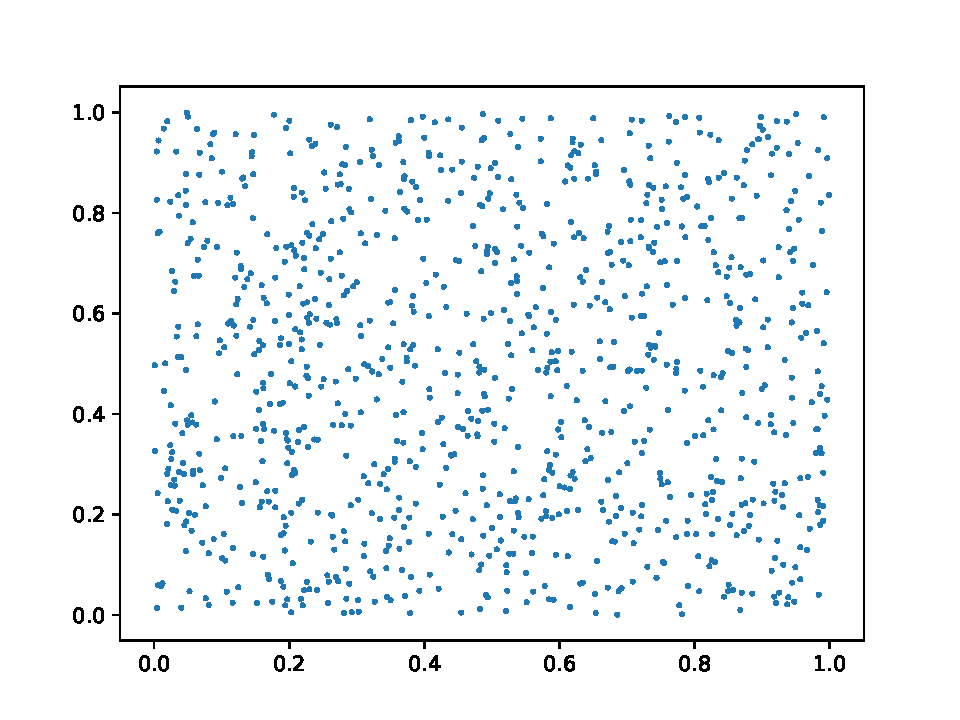
\includegraphics[scale=0.8]{plots/random_next_current.pdf}
\caption{The result of plotting $x_{i+1}$ against $x_i$ for 1000 values. }
\end{figure}
 

\begin{figure}[!hb]
\centering
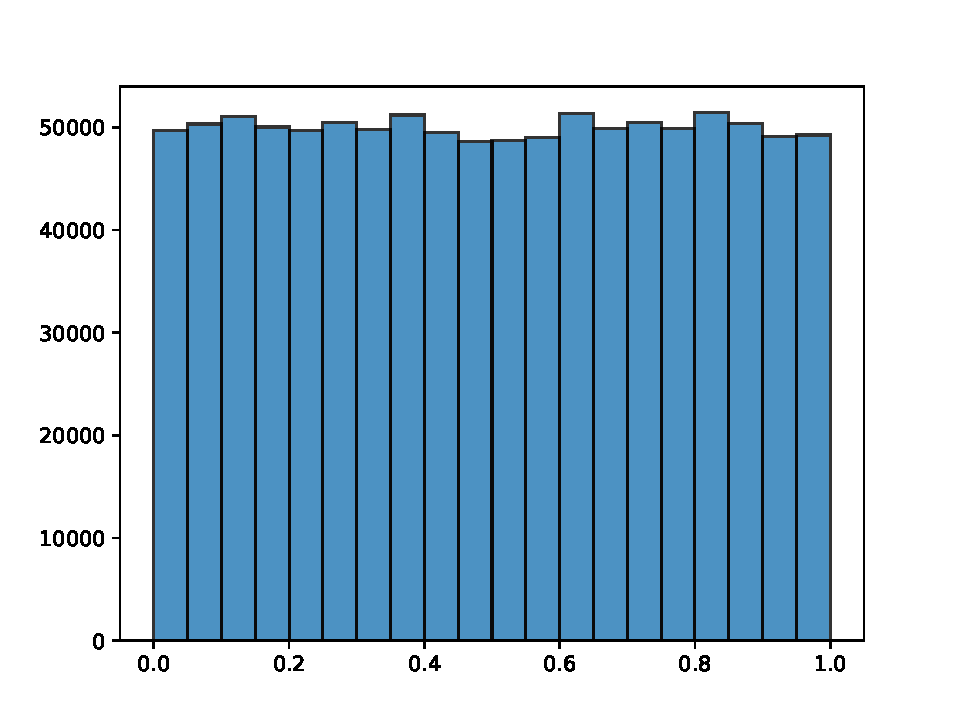
\includegraphics[scale=0.8]{plots/random_uniformness.pdf}
\caption{The uniformness of the random number generator for 1 million generated values between 0 and 1. The values are binned in 20 bins}
\end{figure}
\end{quote}
\newpage
\newpage




%The final output is given by. Here the seed is printed after executing the code as this value will be used for the next exercise (i.e the question was to keep using the same random number generator)
%\lstinputlisting{./assigment1_2_out.txt}









\newpage
\subsection*{Assignment 2.a \hrule}
\textbf{Question}
\begin{quote}
The number density profile for satellite galaxies is given by,
\begin{equation}
n(x) = A \langle N_{sat} \rangle \left(\frac{x}{b} \right)^{a-3} \exp\left[- \left(\frac{x}{b} \right)^c \right]
\end{equation}

where $x$ is the radius relative to the virial radius, and $a$, $b$ and $c$ are free parameters. The value of A here normalizes the integral such that the integral from $x = 0$ to $x = 5$ gives,

\begin{equation}
\langle N_{sat} \rangle= \iiint_V n(x) dV
\label{eq:three}
\end{equation}

Have your code randomly generate three numbers 1.1 $<$ a $<$ 2.5, 0.5 $<$ b $<$ 2 and 1.5 $<$ c $<$ 4. Write a numerical integrator to solve equation \ref{eq:three} in spherical coordinates for A given those three parameters, taking $ \langle N_{sat}\rangle = 100$. Output the numbers a, b, c and A. 

\end{quote}

\textbf{Solution}
\begin{quote}
The value of $A$ is found with the help of Romberg integration. The code for this assignment is located in two files:\textsf{./code/assignment2\_ a.py} and \textsf{./code/mathlib/integrate.py}. The first file contains the code that generates the values $a$, $b$, $c$ and $A$. The second file contains the implementation for Romberg integration. The code for both files and the output can be found below.

\end{quote}

\textbf{Code - output}
\begin{quote}
The code for generating the output.
\lstinputlisting{./code/assignment2_a.py}
\end{quote}

\newpage
\textbf{Code - romberg}
\begin{quote}
The code for romberg integration. 
\lstinputlisting[firstline=0,lastline=76]{./code/mathlib/integrate.py}
\end{quote}

\textbf{Output - Text}
\begin{quote}
The produced output from \textsf{./code/assigment2\_ a.py}.
\lstinputlisting{./output/assignment2_a_out.txt}
\end{quote}











\subsection*{Assignment2.b \hrule}
\textbf{Question}
\begin{quote}
Make a log-log plot of and plot single points for $n(10^{-4})$, $n(10^{-2})$, $n(10^{-1}$), $n(1)$ and $n(5)$ with an axis range from $x = 10^{-4}$ to $x_{max} = 5$. Interpolate the values in between based on just these points - make sure to argue in the comments of your code why you chose to interpolate in a certain way.
\end{quote}

\textbf{Solution}
\begin{quote}
Four out of the 5 points plotted in logarithmic space seems to follow a straight line (see figure 3 below the code section). If we assume that the error on these points is small, then this suggests that the underlying physical relation might be a linear relation in logarithmic space. The last point deviates from this relation with a rapid drop. If we again assume that the error is small, then this suggests that there might be an exponential decrease. 


Most of the data seems to follow a linear relation in log space. If you need to interpolate a value, then you likely need to interpolate withing this linear part, as it wouldn't make much sense to obtained most of your data in a region that is uninteresting. An interpolator should furthermore serve the data  as best as possible. Interpolating the data with a linear and for example a polynomial interpolator, shows that the polynomial interpolator better interpolates the expected exponential drop, where as the linear interpolator better interpolates the expected power law (see figure 4 below the code section). Many other interpolation methods, such as cubic splines and nearest neighbor interpolation, also interpolate the expected exponential drop better than the linear interpolator, but fail to interpolate the linear relation with high accuracy (not shown). 

Based on the above two arguments there is therefore chosen to interpolate the points with a \textbf{linear interpolate} in log space. 


  
The code for this assignment consists of two files: \textsf{./code/assignment2\_ b.py} and   \textsf{./code/mathlib/interpolate.py}. The first file creates the plots and the second file implements the interpolation methods. The code of the two files and the results can be found below.
\newpage
\end{quote}


\textbf{Code - output}
\begin{quote}
The code that interpolates the values and creates the plot.
\lstinputlisting{./code/assignment2_b.py}
\end{quote}

\textbf{Code - interpolate}
\begin{quote}
The code of the linear and polynomial interpolator.
\lstinputlisting{./code/mathlib/interpolate.py}
\end{quote}
\newpage

\textbf{Output - Figure}
\begin{quote}
\begin{figure}[!ht]
\centering
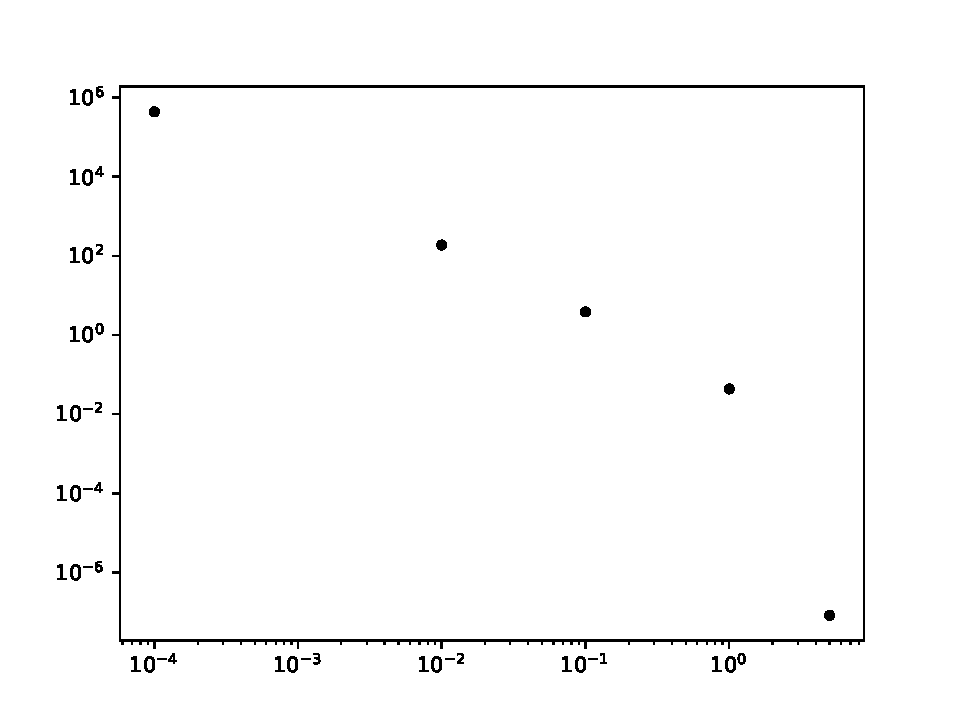
\includegraphics[scale=0.7]{plots/points.pdf}
\caption{A logarithmic plot of the 5 points that need to be interpolated.}
\end{figure}

\begin{figure}[!ht]
\centering
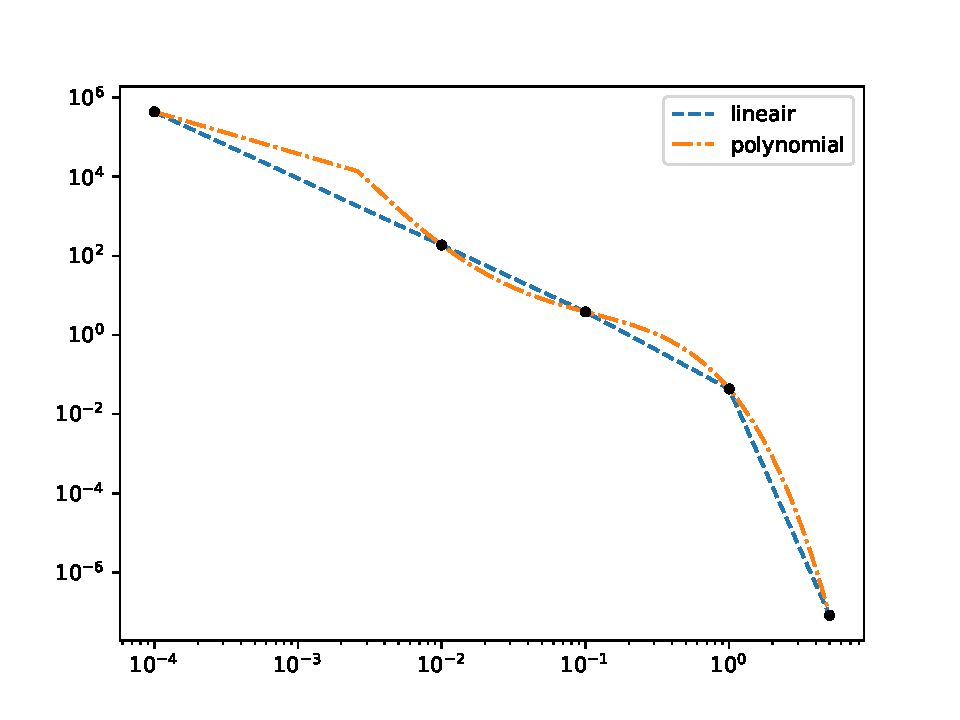
\includegraphics[scale=0.7]{plots/interpolate.pdf}
\caption{The interpolation of the linear interpolator and the polynomial interpolator.}
\end{figure}
\end{quote}
\newpage


 










\subsection*{Assignment 2.c \hrule}
\textbf{Question}
\begin{quote}
Numerically calculate d$n(x)$/dx at $x = b$. Output the value found alongside the analytical result, both to at least 12 significant digits. Choose your algorithm such as to get them as close as possible. 
\end{quote}
\textbf{Solution}
\begin{quote}
The the volume number density for satellite galaxies is,
\begin{equation}
n(x) = A \langle N_{sat} \rangle \left(\frac{x}{b} \right)^{a-3}  \exp\left(-\left(\frac{x}{b} \right)^{c} \right)
\end{equation}

Calculating the analytical derivative gives, 

\begin{align*}
\frac{d n(x)}{dx} &= A \langle N_{sat} \rangle \frac{d}{dx} \left[ \left(\frac{x}{b} \right)^{a-3}  \exp\left(-\left(\frac{x}{b} \right)^{c} \right) \right] \\
&= A \langle N_{sat} \rangle \left((a-3) \left(\frac{x}{b} \right)^{a-4} \frac{1}{b} \exp\left(-\left(\frac{x}{b} \right)^{c} \right) - \left(\frac{x}{b} \right)^{a-3} \exp\left(-\left(\frac{x}{b} \right)^{c} \right)c\left(\frac{x}{b} \right)^{c-1}\frac{1}{b} \right)
\end{align*}
 For $x = b$ this yields,
\begin{equation}
\left.\frac{dy}{dx}\right|_{x=b}  =  A \langle N_{sat} \rangle \left((a-3)e^{-1} \frac{1}{b}-e^{-1} \frac{c}{b} \right) = \frac{A \langle N_{sat} \rangle }{b e} \left((a-3) - c \right)
\end{equation}

The code that calculates the analytical and numerical result consists of two files:  \textsf{./code/assignment2\_ c.py} and \textsf{./code/mathlib/derivative.py}. The first file calculates the analytical and numerical results and outputs these results with 12 significant digits. The second file contains the code for Ridders method, which is used to make the numerical calculation. The code of both files and the output can be found below. 
\end{quote}

\textbf{Code - output}
\begin{quote}
The code that produces the output.
\lstinputlisting{./code/assignment2_c.py}
\end{quote}

\newpage
\textbf{Code - ridder}
\begin{quote}
\hspace*{-0.6cm}The code for ridder's method
\lstinputlisting{./code/mathlib/derivative.py}
\end{quote}

\textbf{Output - Text}
\begin{quote}
The output from \textsf{./code/assignment2\_ c.py} with 12 significant digits.
\lstinputlisting{./output/assignment2_c_out.txt}
\end{quote}
\newpage









\subsection*{Question 2.d \hrule}
\textbf{Question}
\begin{quote}
Now we want to generate 3D satellite positions such that they statistically follow the satellite profile in equation (2) of the assignment; that is, the probability distribution of the (relative) radii $x \in [0, x_{max})$ should be $p(x)dx = n(x)4\pi x^2 dx/ \langle N_{sat} \rangle$ (with the same a,b and c as before). Use one of the methods discussed in class to sample this distribution. Additionally, for each galaxy generate random angles $\phi$ and $\theta$ such that the resulting positions are (statistically) uniformly distributed as a function of direction. Output the positions ($r, \phi, \theta$) for 100 such satellites.
\end{quote}

\textbf{Solution} 
\begin{quote}
Let $v$ be a uniform random variable between 0 and 1. A uniform distributed $\phi$ and $\theta$ on a sphere are then given by,

\begin{align}
\phi &= 2 \pi v \\
\theta &=  \arccos(1-2v)
\end{align}

These equation can be derived from a uniform distribution for the solid angle. This derivation is not asked in the question and the equations are therefore directly taken from the first slide of the 5th lecture.

The radius $x$ is sampled from the given probability distribution $p(x) = n(x)4 \pi x^2/ \langle N_{sat} \rangle$ with the help of rejection sampling. To apply rejection sampling first a distribution $p_{enc}(x)$ is chosen that encloses all of $p(x)$ when the distribution is multiplied with a scalar $k$ (i.e $p(x) < kp_{enc}(x) \ \forall \ x \in[0,5)$). The chosen distribution is an uniform distribution for $x \in[0,5)$,
\begin{equation}
p_{enc}(x) = 
     \begin{cases}
       \frac{1}{5} &\quad\text{for $0< x < 5$} \\
       0  &\quad\text{otherwise}
     \end{cases}
\end{equation}  

The scalar is chosen to be $k = 2$. To apply rejection sampling it must first be possible to generate samples from $p_{enc}$. To sample from this distribution the fundamental transformation law of probability is applied. Let $y$ be a uniform random variable between 0 and 1.  Let $z$ be distributed according to $p_{enc}$. The fundamental transformation law of probabilities then yields, 
\begin{equation}
\int_0^z p_{enc}(z') dz' = \int_0^y 1 dy' 
\end{equation}

Solving this for $z$ gives the transformation that is needed to let $Y$ be distributed according to $p_{enc}$,
\begin{equation}
 z = 5y
\end{equation}

%The variable $y$ can be generated from the random number generator and the above transformation allows us to transform it to a sample distributed according to $p_{enc}$. 

Samples distributed according to $p(x)$ can now be found with rejection sampling:  Generate a random uniform variable $y$ between 0 and 1. Transform this variable to obtain a random variable z distributed according to $p_{enc}$. If a new random variable $w$ generated\footnote{Let $u$ be an uniform variable between 0 and 1, then w is given by $w = k*p_{enc}(z)*u$. This can be derived on exactly the same way as equation 10.} from an uniform distribution between 0 and $k p_{enc}(z)$  is smaller or equal than $ p(z)$, then $z$ is a sample from the distribution of which we want to sample. If the condition does not hold reject the sample and repeat the above process.    



The code used for the sample generation and the printing of the results consists of two files. The first file is the file that prints the results: \textsf{./code/assignment2.d.py}.  The second file, \textsf{./code/mathlib/rng.py}, contains the functions \textsf{rejection\_ sample} and \textsf{gen\_ uniform\_ spherical\_ surface\_ coords}) that are used to obtain the result. \textbf{The code for the second file can be found on pages 6 and 7}. The code for the first file and its output can be found on the next page.


\end{quote}

\textbf{Code - output}
\begin{quote}

The code that generates the output. 
\lstinputlisting{./code/assignment2_d.py}
\end{quote}

\textbf{Output - text}
\begin{quote}
The generated output.
\lstinputlisting{./output/assignment2_d_out.txt}
\end{quote}












\subsection*{Assignment 2.e \hrule}
\textbf{Question}
\begin{quote}
Repeat the previous exercise for 1000 haloes each containing 100 satellites. Make another log-log plot showing $N(x) = n(x)4 \pi x^2$ over the same range as before, but now over-plot a histogram showing the average number of satellites in each bin. Use 20 logarithmically-spaced bins between $x = 10^{-4}$ and $x_{max}$ and don't forget to divide each bin by its width. Do you generated galaxies match this distribution?
\end{quote}


\textbf{Solution}
\begin{quote}
The histogram with the average number of satellites is created by first creating a histogram for each halo and adding each of these histograms together. The obtained "super" histogram is next divided by the width of the bins to correct for the different sized bins. The bin width corrected "super" histogram is finally divided by the number of halos to obtain the histogram with the average number of satellites. 

The code that generates the radii and the histogram is located in the file: \textsf{./code/assignment2\_ e.py}. The content of this file and its output can be found below\footnote{The code of the helper functions used in this file can be found in the previous assignment.}. The output is located at

\end{quote}
  
\textbf{Code - plots}
\begin{quote}
\lstinputlisting{./code/assignment2_e.py}
\end{quote}

\textbf{Output - plot}

\begin{quote}
The output generated by \textsf{./code/assignment2\_ e.py} consists of figure \ref{fig:sat} on the next page.
\newpage
\begin{figure}[!ht]
\centering
\vspace*{-1cm}
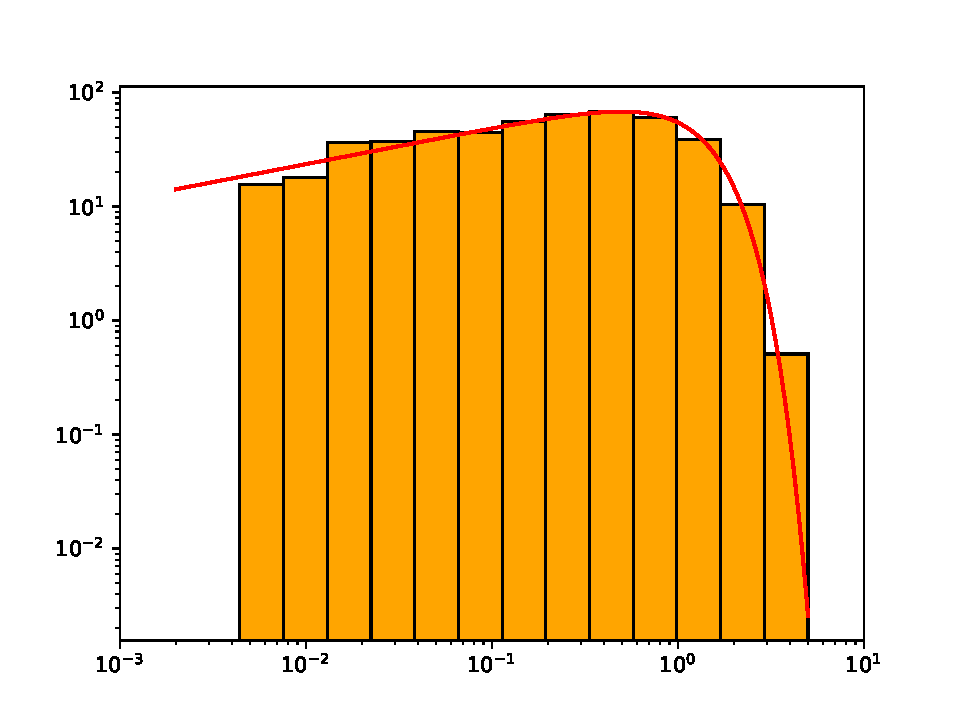
\includegraphics[width=12cm, height=8.5cm]{plots/assignment2e.pdf}
\caption{The average number of satellites on a spherical shell at distance $x = r/r_{viral}$. The red line is the original function $N(x)$ that is used to generate the histogram.}
\label{fig:sat}
\end{figure}
\end{quote}












\subsection*{Assignment 2.f \hrule}

\textbf{Question}
\begin{quote}
Write a root-finding algorithm to find the solution(s) to $N(x) = y/2$ in the same x-range, where $y$ is the maximum of $N(x)$. Use the same parameter values as before. Output the root(s).
\end{quote}

\textbf{Solution}
\begin{quote}
The x-c\" oordinate of the maximum is determined analytically by taking the derivative of $N(x)$,
  
\begin{align*}
\frac{d N(x)}{dx} &= 4 \pi A \langle N_{sat} \rangle \frac{d}{dx} \left[b^2 \left(\frac{x}{b} \right)^{a-1}  \exp\left(-\left(\frac{x}{b} \right)^{c} \right) \right] \\
&= 4 \pi A \langle N_{sat} \rangle \left(b^2 (a-1) \left(\frac{x}{b} \right)^{a-2} \frac{1}{b} \exp\left(-\left(\frac{x}{b} \right)^{c} \right) - b^2\left(\frac{x}{b} \right)^{a-1} \exp\left(-\left(\frac{x}{b} \right)^{c} \right)c\left(\frac{x}{b} \right)^{c-1}\frac{1}{b} \right) \\
&= 4 \pi \langle N_{sat} \rangle b \exp \left(- \left(\frac{x}{b}\right)^c \right)
 \left( (a-1) \left(\frac{x}{b} \right)^{a-2} - c\left( \frac{x}{b} \right)^{a-1} \left(\frac{x}{b} \right)^{c-1} \right)
\end{align*}

Equating the derivative to zero gives as solutions that,  
\begin{equation}
4 \pi \langle N_{sat} \rangle b \exp \left(- \left(\frac{x}{b}\right)^c \right) = 0\hspace*{0.5cm} \text{or} \hspace*{0.5cm}  \left( (a-1) \left(\frac{x}{b} \right)^{a-2} - c\left( \frac{x}{b} \right)^{a-1} \left(\frac{x}{b} \right)^{c-1} \right) = 0
\end{equation}

The equation on the left is not solvable. Taking the equation on the right and solving it for x gives,
%Simplifying then yields,
\begin{align*}
(a-1) \left(\frac{x}{b} \right)^{a-2} &= c\left( \frac{x}{b} \right)^{a-1} \left(\frac{x}{b} \right)^{c-1} \\
(a-1) \left(\frac{x}{b} \right)^{a-2} &= c\left( \frac{x}{b} \right)^{a-2} \left(\frac{x}{b} \right)^{c} \\
(a-1) &= c \left(\frac{x}{b} \right)^{c} \\
x_{max} &= \left( \frac{a-1}{c} \right)^{1/c} b
\end{align*}

The maximum value, $y$, is now given by,
\begin{equation}
y = N(x_{max})
\end{equation}


The roots of $N(x) - y/2 = 0$ are found with the Newton-Raphson method. The code that applies the Newton-Raphson method and prints the root is located in the file: \textsf{./code/assignment2\_ f.py}. The implementation of the Newton-Raphson method  is found in \textsf{./mathlib/roots.py}. The content of these files and the output of the first file can be found below. % code files and the output of the first file is shown below.
\end{quote}

\textbf{Code - output}
\begin{quote}
The code that find the roots and prints them.
\lstinputlisting{./code/assignment2_f.py}
\end{quote}

\textbf{Code - Newton- Raphson}
\begin{quote}
The code for the Newton-Raphson method.
\lstinputlisting[lastline=61]{./code/mathlib/roots.py}
\end{quote}

\textbf{Output - text}
\begin{quote}
The output of \textsf{./code/assigment2\_ f.py}
\lstinputlisting{./output/assignment2_f_out.txt}
\end{quote}



 







\subsection*{Assignment 2.g \hrule}
\textbf{Question}
\begin{quote}
Take the radial bin from assignment 2.e containing the largest number of galaxies. Using sorting, calculate the median, 16th and 84th percentile for this bin and output these values. Next, make a histogram of the number of galaxies in this radial bin in each halo (so 1000 values), each bin of this histogram should have a width of 1. Plot this histogram, and over-plot the Poisson distribution with $\lambda$ equal to the mean number of galaxies in this radial bin.
\end{quote}

\textbf{Solution}
\begin{quote}

The code does for this exercise  consists of three files. The first file (\textsf{./code/assignment2\_ g.py}) contains the code that creates the plot and prints the output. The second file (\textsf{./code/mathlib/sorting.py}) contains the code for merge sorting. The last file (\textsf{./code/mathlib/utils.py}) contains the functions for the median, percentile and Poisson distribution. A part of this last file has earlier been shown in assignment 1.b. The full file, inclusive the earlier shown part, can be found below. 

% and the percentile. This last file also contains other functions that have previously bee 
%n the array of the 84 th percentile is not an integer (i.e index = 5.54), then lineair interpolate the value at index 5 and at index 6 to estimate the value at index 5.54. 
\end{quote}
\newpage

\textbf{Code - output}
\begin{quote}
The code that produces the output.
\lstinputlisting{./code/assignment2_g.py}
\end{quote}

\textbf{Code - merge sort}
\begin{quote}
The code for merge sort that is used for the median and the percentile.
\lstinputlisting[lastline=71]{./code/mathlib/sorting.py}
\end{quote}

\textbf{Code - Poisson, median, percentile}
The code of the Poisson distribution, median function and percentile function.
\begin{quote}
\lstinputlisting{./code/mathlib/utils.py}
\end{quote}

\textbf{Output - text}
\begin{quote}
The text output from \textsf{./code/assignment2\_ g.py}
\lstinputlisting{./output/assignment2_g_out.txt}
\end{quote}

\newpage

\textbf{Output - figure}
\begin{quote}
The plot created in \textsf{./code/assignment2\_ g.py}
\begin{figure}[!h]
\centering
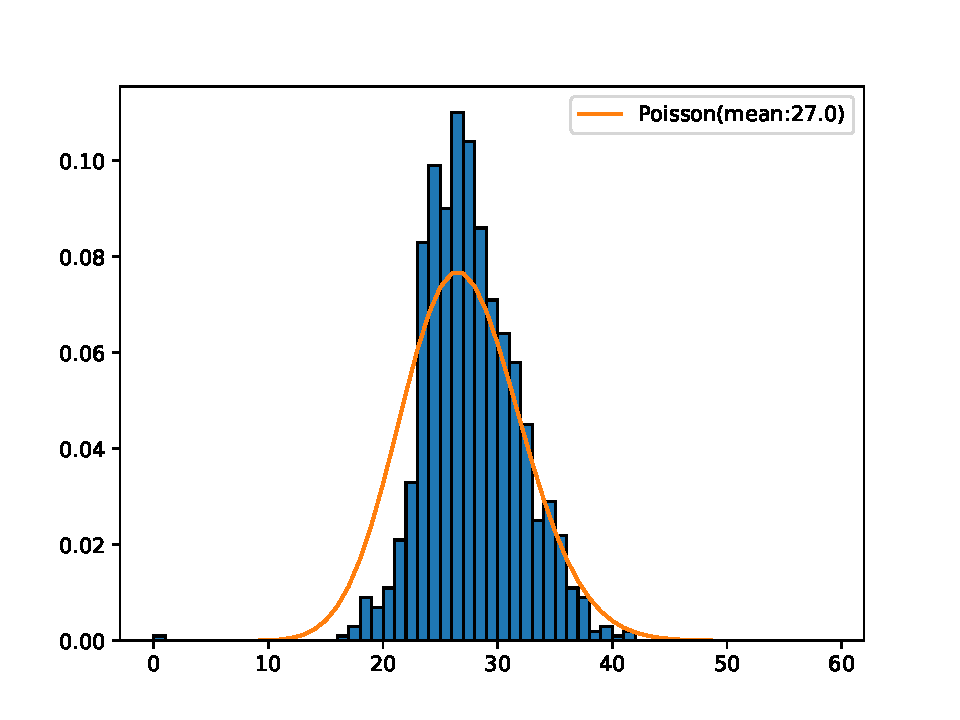
\includegraphics[scale=0.7]{plots/poisson.pdf}
\caption{The Poisson distribution over-plotting the created histogram. The figure shows that the number of satellites on a spherical shell at a distance x is approximately distributed according to a Poisson distribution around N(x) - the number of satellites predicted by the model on an infinite thin spherical shell. }
\end{figure}
\end{quote}













\subsection*{Question 2.h \hrule}
\textbf{Question}
\begin{quote}
The normalization factor $A$ depends on all three parameters. Calculate $A$ at 0.1 wide intervals in the range of $a$, $b$ and $c$ given above (including the boundaries). You should get a table containing 6240 values. Choose an interpolation scheme and write a 3D interpolator for $A$ as a function of the three parameters based on these calculated values.
\end{quote}

\textbf{Solution}
\begin{quote}
The chosen interpolator is a 3D linear interpolator. The code for the interpolator and the explanation of how it interpolates can be found in the  file \textsf{./code/mathlib/interpolate3D.py}.  The file makes use of 1 dimensional linear interpolator of which the code can be found in question 2.b. The code that creates the table can be found in the file \textsf{./code/assignment2\_ h.py}. 
\end{quote}
\newpage

\textbf{Code - Table}
\begin{quote}
The code that creates the table and performs a small test to see how well 
the interpolator approximates the true value.
\lstinputlisting{./code/assignment2_h.py} 
\end{quote}

\textbf{Code - interpolator}
\begin{quote}
The code for the 3D interpolator
\lstinputlisting{./code/mathlib/interpolate3D.py} 
\end{quote}


\newpage











\subsection*{Assignment 3.a \hrule}
\textbf{Question}
\begin{quote}
Download the provided file. Each file contains haloes in a certain mass bin with variable numbers of satellites. Write down the log-likelihood corresponding to a set of random realizations of the satellite profile with some unknown $\langle N_{sat} \rangle$. Retain only the terms with a (residual) dependence on a, b and/or c (including A = A(a, b, c)). 

Find the a, b and c that maximize this likelihood. Do this separately for each different file/mass
bin. Output these values.
\end{quote}

\textbf{Solution}
\begin{quote}
Recall that the number of satellites predicted by the model on an infinite thin spherical shell at a distance x is given by,

\begin{equation}
N(x) = 4\pi A \langle N_{sat} \rangle b^{2} \left(\frac{x}{b} \right)^{a-1} \exp \left[-\left(\frac{x}{b} \right)^c \right]
\label{eq:N}
\end{equation}

here $\langle N_{sat} \rangle$ is the total amount of satellites in the halo and $A$ is a normalization constant such that the integral from $x = 0$ to $x = x_{max}$ of $N(x)$ is $\langle N_{sat} \rangle$.

In exercise 2.g it was found that the number of satellites on a sphere shell at distance $x$ is approximately distributed according to a Poisson distribution around N(x). If we assume that the distribution of satellites for haloes in the same mass bin is similar, then the probability to find the data in one of the files given the model is given by,
\begin{equation}
P(\text{data}|\text{model}) = \prod_{i=0}^{N-1} \frac{N(x_i | a, b, c)^{y_i} e^{-N(x_i | a, b, c)}}{y_i!}
\end{equation}

here $x_i$ is the distance to a satellite, $y_i$ is the number of satellites at this distance.  The optimal value's of $a$, $b$ and $c$ that maximize this probability can be found minimizing the negative log-likelihood,
\begin{equation}
- \ln(P(\text{data}|\text{model})) = -\sum_{i = 0}^{N-1} \left[ y_i \ln(N(x_i | a, b, c)) -N(x_i | a, b, c) - \ln(y_i!) \right]
\label{eq:non_assum}
\end{equation}

The satellites in the haloes of the same mass bin are, as mentioned before, expected to have the same distribution. The data of the haloes of a single file is therefore combined to create a super halo.  It is next assume that in the super halo has an infinite amount of bins.  In this case $y_i$ is either 0 or 1 and the negative log-likelihood then becomes,
\begin{equation}
- \ln(P(\text{data}|\text{model})) \approx \sum_{i=0}^{M-1} \left[- \ln(N(x_i | a, b, c)) \right] + \int_0^{x_{max}} N(x | a, b, c) dx
\end{equation}

here the sum is taken over the $M$ positions of the  satellites in the super halo. The integral over all radii is however equal to the total number of satellites in the super halo and the function to minimize therefore becomes,

\begin{equation}
- \ln(P(\text{data}|\text{model})) \approx \sum_{i=0}^{M-1} \left[- \ln(N(x_i | a, b, c)) \right] +\langle N_{sat} \rangle
\end{equation}


This function is minimized with the help of the downhill simplex method. The function is minimized withing a bounded interval: $1.1 \leq a \leq 2.5$, $0.5 \leq b \leq 2$, $1.5 \leq c \leq 4.0$. The value of $x_{max}$ is furthermore chosen to be 5. These choices make it possible to use the interpolator of the previous question to determine the value of the normalization constant $A(a, b, c)$. The value of $\langle N_{sat} \rangle$ is for each super halo set to the total amount of satellites in the super halo. The log likelihood function is finally slightly modified to prevent any minimization algorithm from walking outside the bounces. If a minimization algorithm tries an parameter that is outside one of the bounces, then the parameter will be set to the value of the bounce before evaluating the log likelihood (i.e if the downhill simplex method  tries $a = 0.47$ then $a$ is first set to 0.5 before evaluating the log likelihood).



The code that finds the optimum values of $a$, $b$ and $c$ is located in 3 files:
\textsf{./mathlib/code/assignment3.a.py},  \textsf{./mathlib/code/minimise.py}, \textsf{./mathlib/code.interpolate.py}. The first file finds the optimal values of $a$, $b$ and $c$ for each mass bin. The second file contains the implementation of the downhill simplex method. The last file contains the code for the interpolator. The produced output of the code and the code in the first two files can be found below. The code for the last file can be found in the previous assignment. 

\end{quote}


\textbf{Code - output}
\begin{quote}
\lstinputlisting{./code/assignment3_a.py}
\end{quote}

\textbf{Code - downhill}
\begin{quote}
\lstinputlisting{./code/mathlib/minimize.py}
\end{quote}

\textbf{Output - text}
\begin{quote}
The optimal values found by \textsf{./mathlib/code/assignment3.a.py}:
\lstinputlisting{./output/assignment3_a_out.txt}
\end{quote}

\textbf{Output - plots}
\begin{quote}
The fit of equation \ref{eq:N} to the data in the different files for the found optimal values. 

\begin{figure}[!h]
\centering
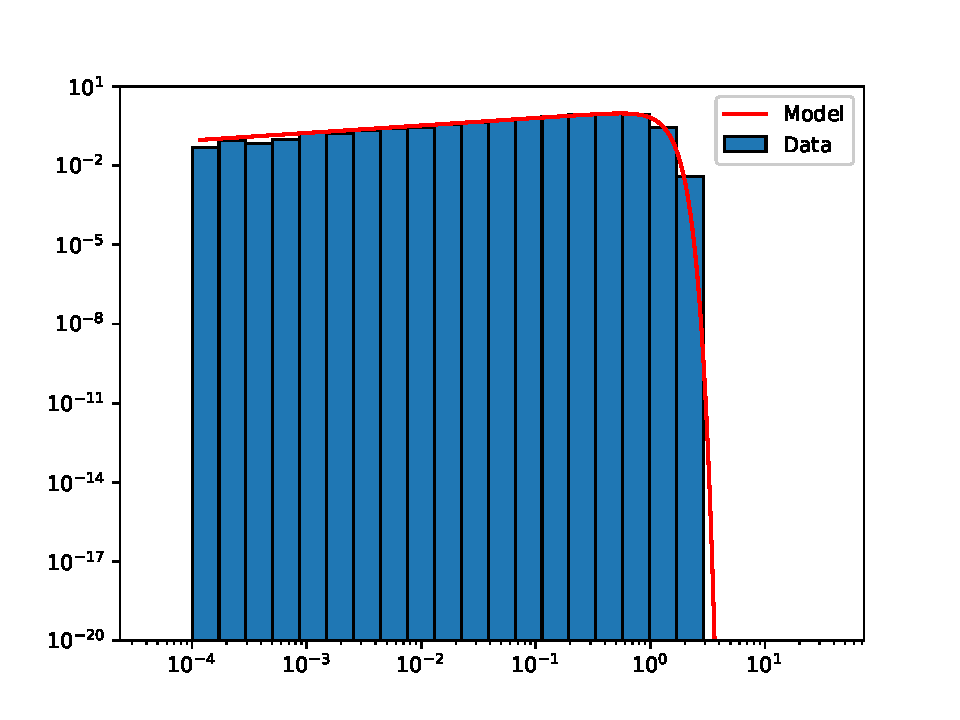
\includegraphics[scale=0.7]{plots/satgals_m11.pdf}
\caption{The model (equation \ref{eq:N}) with the found parameters of $a$, $b$ and $c$ fitted to the data for the mass bin of $10^{11}$ $M_{\odot}$.}

\end{figure}
\newpage

\begin{figure}[!h]
\centering
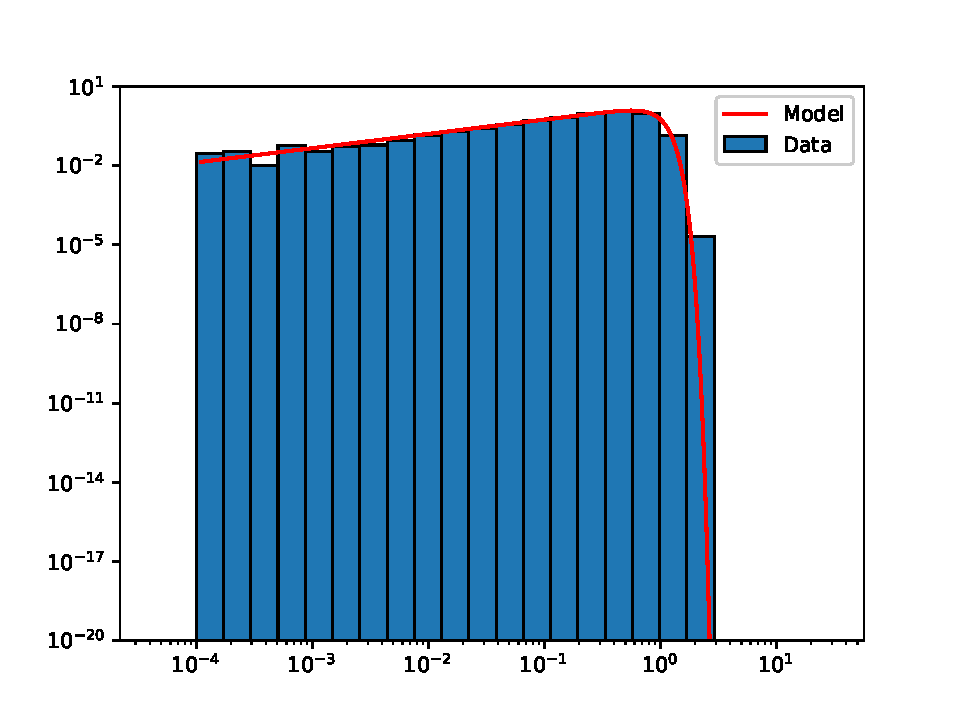
\includegraphics[scale=0.7]{plots/satgals_m12.pdf}
\caption{The model (equation \ref{eq:N}) with the found parameters of $a$, $b$ and $c$ fitted to the data for the mass bin of $10^{12}$ $M_{\odot}$.}

\end{figure}

\begin{figure}[!ht]
\centering
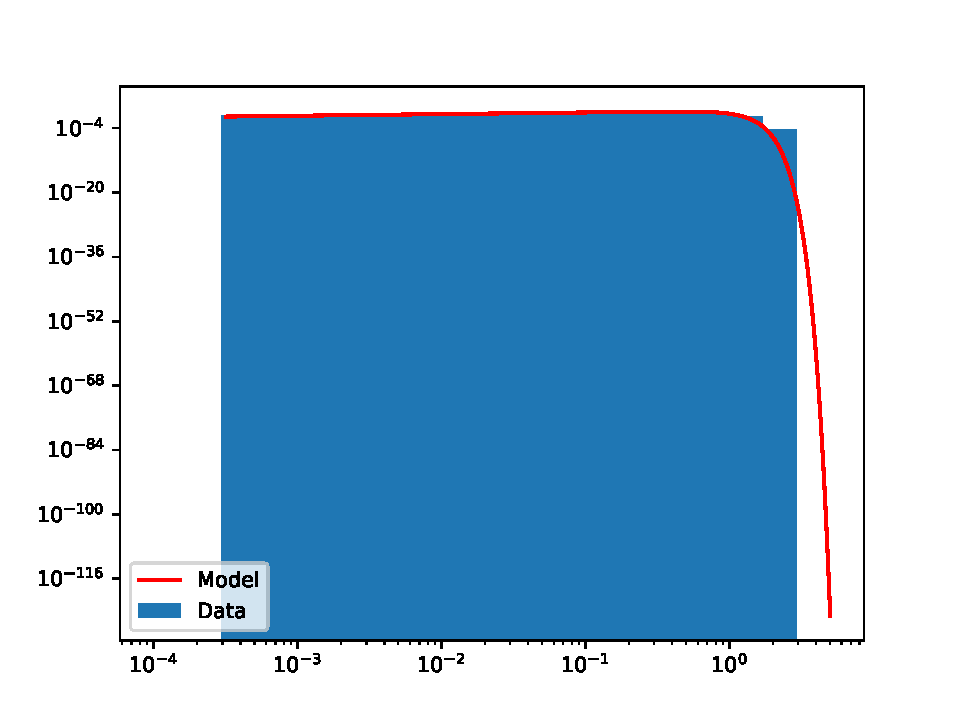
\includegraphics[scale=0.7]{plots/satgals_m13.pdf}
\caption{The model (equation \ref{eq:N}) with the found parameters of $a$, $b$ and $c$ fitted to the data for the mass bin of $10^{13}$ $M_{\odot}$.}
\end{figure}
\newpage
\begin{figure}[!hb]
\centering
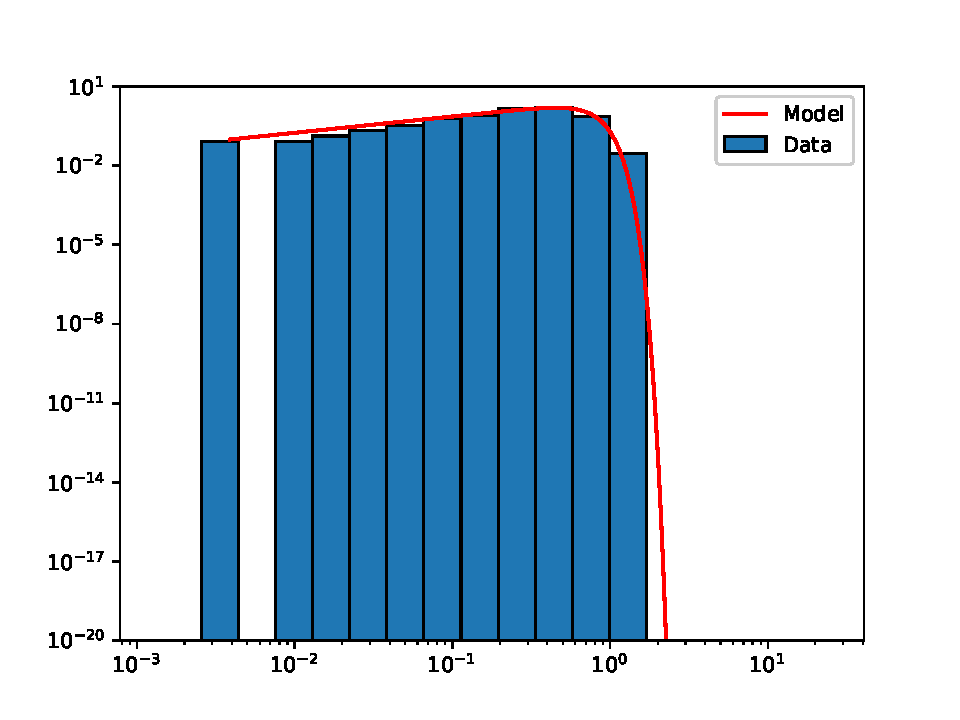
\includegraphics[scale=0.7]{plots/satgals_m14.pdf}
\caption{The model (equation \ref{eq:N}) with the found parameters of $a$, $b$ and $c$ fitted to the data for the mass bin of $10^{14}$ $M_{\odot}$.}
\end{figure}


\begin{figure}[!ht]
\centering
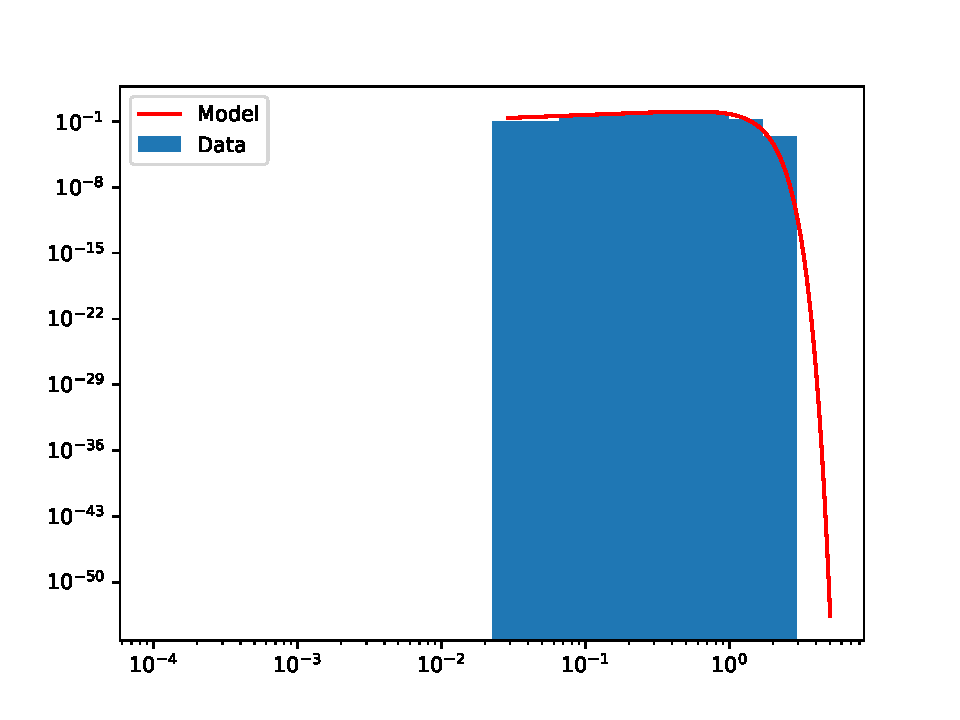
\includegraphics[scale=0.7]{plots/satgals_m15.pdf}
\caption{The model (equation \ref{eq:N}) with the found parameters of $a$, $b$ and $c$ fitted to the data for the mass bin of $10^{15}$ $M_{\odot}$.}
\end{figure}
\end{quote}
\newpage





















  







\end{document}
